\label{chpt:modelling and techniques} % for referencing this chapter elsewhere, use 
\lhead{\emph{Modelling, techniques, and methods}} % This is for the header on each page - perhaps a shortened title


% In the preamble, give the short version of "we can extract a lot of data from eclipsing CVs" etc.
% Also bring up that, because a CV is so compact, the population of eclipsers is actually fairly high.
% Talk about the state of stellar modelling, and say that we can apply it to CVs. Talk about how we can use this to convert eclipse modelling characterisation directly to an empirical mass loss rate, slash AML rate.

The primary goal of this thesis is to characterise as many CVs as possible. In this work, I am primarily interested in finding independant measures of the donor mass and radius, measurements of the white dwarf mass and radius, and the orbital separation between the two. These metrics provide valuable probes of CV evolution \citep{knigge2006}, which is explored more thoroughly in \S\ref{sect:method:evolutionary modelling}. 
This chapter describes in detail the two modelling techniques used for this thesis: the characterisation of a CV using multi-band eclipse modelling, and inferring the long-term mass loss rate of a system from its donor properties.


\section{Calculating orbital ephemerides}
\label{sect:modelling:calculating ephemeris}

Crucial to both observing and modelling an eclipse is a good knowledge of the orbital ephemeris. This is described by the equation
\begin{equation}
    \label{eqn:modelling:general ephemeris equation}
    T_{\rm ecl} = T_0 + P_{\rm orb} E
\end{equation}
where $T_{\rm ecl}$ is the time of mid-eclipse, $T_0$ is the mid-eclipse time of the zeroth eclipse, and $E$ is the eclipse number. Accurately calculating $T_{\rm ecl}$ is important to scheduling observations of a system, and $P_{\rm orb}$ is a crucial input to the eclipse modelling that I later conduct. 

A very high accuracy in $P_{\rm orb}$ is important, as observations are often separated by several months or even years, and an error of even $\sim 0.1$ seconds can accumulate to give incorrect predicted eclipse times. This need for accuracy and precision also requires the definition of {\it where} a time is recorded from. All eclipse times presented in this thesis are given in the Barycentric Modified Julian Date (BMJD), which is the time of eclipse as measured from the centre of mass of the solar system. Note that this is different to the heliocentric MJD often seen in the literature, as the location of the sun deviates from the centre of mass. Where heliocentric literature values are used, they are first converted to BMJD. 

Simply taking a time of minimum light is insufficient for the systems in this work, as it is common for these eclipses to have very flat eclipse minima. A somewhat more sophisticated method is necessary.

Finding the mid-eclipse time was done by looking at the numerical derivative of an eclipse. 
First, an eclipse is smoothed to remove short term fluctuations, mostly those due to noise but also to partly mitigate the short term flickering often seen in CVs. This initial smoothing was done by applying a median filter to the data. Then, the numerical derivative is calculated and smoothed again, this time with a `boxcar' convolution. Properly filtered, the dominant remaining features of the numerical derivative are the ingresses and egresses of the white dwarf and bright spot. 
The white dwarf ingress and egress are, in theory, mirror images of one another. The ingress should be a sharp, negative spike, and egress should be a sharp, positive spike. As the two should be the same shape, a double-gaussian is fit to the derivative, using manually chosen initial conditions. In this model, the two gaussians share a width, $\sigma$, and have their mid-points described by
\begin{align*}
    T_{\rm 1,2} = T_{\rm ecl} \pm \Delta T
    h_{\rm 1,2} = \pm h
\end{align*}
where $T_{1,2}$ are the midpoints of the two gaussians, $h_{1,2}$ are their heights, and $2\Delta T$ is the width of the white dwarf eclipse. Four important free parameters are then fitted to the data, $T_{\rm ecl}$, $\sigma$, $h$, and $\Delta T$. 

To find a rough initial ephemeris of a system, at least two eclipse observations with known $E$ are necessary. Given no prior knowledge of $P_{\rm orb}$ and $T_0$, this can be done by simply observing the system for several hours, until two consecutive eclipses are seen. This gives a rough measure of $P_{\rm orb}$, but can be significantly refined with longer baseline observations. 
For each observed $T_\mathrm{ecl}$, $E$ could unambiguously be determined, either from observing consecutive eclipses or from previously reported literature values.
An MCMC algorithm was used to fit a straight line model to the independent variable $E$\ and dependent variable $T_\mathrm{ecl}$, with a gradient $P$\ and intercept $T_0$. 
The model also accounts for potential systematic differences in timing accuracy between instruments by also having variable error scale factors applied to all eclipses observed with a specific instrument, e.g. the timing reported for eclipses observed with ULTRACAM may be systematically offset from reality, and the errors associated with those observations might need to be larger than reported to be consistent with data from other instruments. The prior distribution assumed for these error factors was log-uniform ranging from 0.01 to 100, which favours the smallest factor consistent with the data. 

The values of $E$ for each system were chosen to minimise the covariance between $T_0$ and $P$. 
\todo{Should I explain the covariance minimisation algebra?}
If we consider the result of fitting  $T_0, P_{\rm orb}$ as a multivariate normal, $N(\mu, \Sigma)$, we can write
\begin{align}
    \mu =& 
    \begin{pmatrix}
        T_0 \\
        P_{\rm orb}
    \end{pmatrix}
    \\
    \label{eqn:modelling:ephemeris multivariate normal}
    \Sigma =& 
    \begin{pmatrix}
        \sigma_{\rm T0}^2 & \sigma_{\rm T0} \sigma_{\rm P} \\
        \sigma_{\rm P} \sigma_{\rm T0} & \sigma_{\rm P}^2  \\
    \end{pmatrix}
\end{align}
Now, consider a predicted eclipse time for $E$. The uncertainty in Equation~\ref{eqn:modelling:general ephemeris equation} can be written as,
\begin{equation}
    \sigma_T^2 = \sigma_{\rm T0}^2 + 2\sigma_{\rm T0} \sigma_{\rm P}E + \sigma_{\rm P}^2 E^2
\end{equation}
from the standard error propagation formula.
$E$ can be offset by some integer, $N$, as $E' = E - N$. Then, by expanding out the brackets and consolidating some terms, $\sigma_T^2$ becomes
\begin{align*}
    \sigma_T^2 =& \sigma_{\rm T0}^2 + 2\sigma_{\rm T0} \sigma_{\rm P}(E'+N) + \sigma_{\rm P}^2 (E'+N)^2 \\
    =& (\sigma_{\rm T0}^2 + \sigma_{\rm P}^2 N^2 + 2\sigma_{\rm T0} \sigma_{\rm P} N) + 2(\sigma_{\rm T0} \sigma_{\rm P} + \sigma_{\rm P}^2 N)E' + \sigma_{\rm P}^2 E'^2
\end{align*}
Since we want to minimise the $\sigma_T^2$ term, we can choose a value of $N$ to do so, $N = -(\sigma_{\rm T0}\sigma_{\rm P})/(\sigma_{\rm P}^2)$ rounded to the nearest integer.


\section{Eclipse modelling of a CV}
\label{sect:method:lightcurve modelling}

To determine the system parameters for the three CVs in this study, the eclipse lightcurves were modelled. This method is more frequently applicable in CVs than the more traditional approach of using spectroscopic eclipsing binaries, since the donor star is rarely directly visible. Compared to using the superhump period excess to estimate the mass ratio \citep{patterson2005, knigge2006}, lightcurve modelling requires few assumptions. However, it does require precise alignment of the system and so is not possible for a large fraction of CVs.

CV eclipse modelling was first developed by \citet{wood1986}, and has been refined significantly over the last decade \citep{Savoury2011, McAllister2017, McAllister2019}. This method relies of four assumptions: the bright spot originates where a ballistic trajectory from the donor meets the outer edge of the accretion disc, the white dwarf obeys a theoretical mass-radius relationship, the white dwarf is unobscured by the accretion disc or other sources of intra-system material, and the donor exactly fills its Roche lobe. Most of these assumptions are considered robust, though the visibility of the white dwarf been called into question by \citet{Spark2015}.

Recall that the light from a CV originates from four distinct objects in the system. The white dwarf and donor star, the accretion disc about the white dwarf, and the bright spot impact region (hereafter simply `the bright spot'), where transferred material impacts the outer rim of the accretion disc and liberates significant amounts of energy.
The anatomy of a CV lightcurve as the donor star eclipses the other components in the system is comprised of XX events, that occur in the following order:
\begin{enumerate}
    \item a 
\end{enumerate}



\subsection{Capturing flickering with Gaussian Processes}
Explain GPs from scratch, and get into detail about which kernels you're using. 


\section{The optimisation problem}
Here I should discuss the problem of searching 15 dimensions for the best solution - then point out how much worse it is with 100+ dimensions. Here, I should put in some illustrative model fitting - perhaps a graph with steps vs. ln(like) for 1D, 5D, 10D, 15D? Dunno yet. Think about it. Alternatively, just make "MCMC Fitting" the section heading, and get straight into it. Mention binning eclipse lightcurves here as a primary mitigation strategy for the highly complex parameter space


\subsection{Hierarchical model structure}
{\bf This is going to take some work. Fit synthetic lightcurves with various amounts of noise, (5\%, 10\%, 20\%?), and compare convergence times and posterior widths as a function of noise. Do this with one eclipse, then with three eclipses of the same band, then with three eclipses in each of three bands.
I should see an improvement in final probability distribution with more eclipses, since they can communicate.
Also, I need to come up with a way to demonstrate the potential to break degeneracies. Some lightcurves might be produced by two different parameter vectors, e.g. disc and donor might look similar to each other. }

I extend the lightcurve fitting model used by \citet{McAllister2019}, adopting a hierarchical approach to slightly reduce model complexity. 

Changes in the disc radius and brightness profile, and bright spot parameters can mean that the same CV has a significantly different eclipse lightcurve at different times, making it difficult to justify averaging together many eclipses, as features can become smeared out and uninformative. In the worst-case scenario, all 18 parameters would be independently variable for each eclipse, in each band. However, by sharing some parameters between eclipses and bands, this large number of free parameters is slightly reduced, and the posterior of some parameters can be informed by multiple eclipses. \citet{McAllister2017} share $q,\ R_{\rm WD}/a$, and $\Delta\phi$ between eclipses, and we extend that concept by organising the model into a hierarchical tree structure, a schematic of which is shown in Figure~\ref{fig:method:hierarchical_model}. 

\begin{figure}
    \centering
    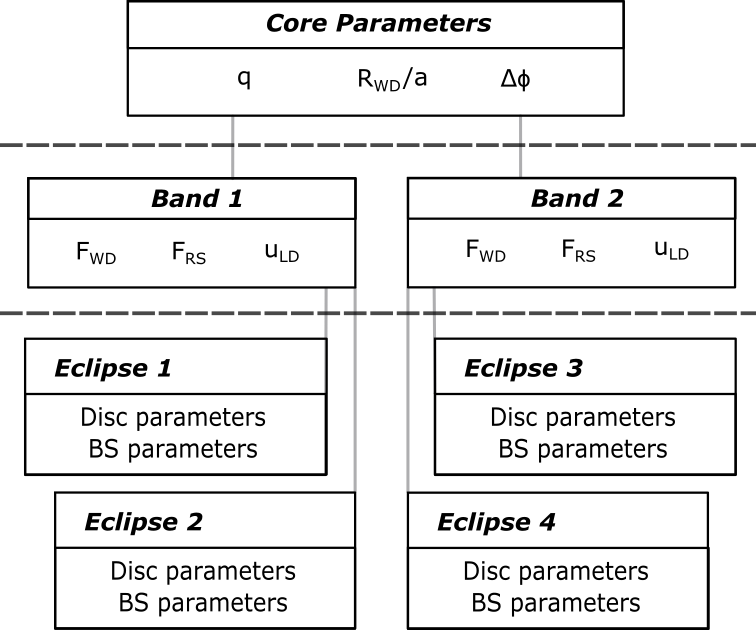
\includegraphics[width=.85\columnwidth ]{figures/three_cvs_with_weird_colours/GeneralFigs/hierarchical_model_structure.png}
    \caption{The hierarchical structure of the lightcurve model. Parameters are inherited downwards, to produce an eclipse at the `leaves' of the tree, e.g. Eclipse 3 inherits the parameters of Band 2, which in turn inherits the Core parameters. $\mathrm{F_{WD, RS}}$\ represent the fluxes of the white dwarf and donor star, and $\mathrm{U_{LD}}$\ is the limb darkening coefficient of the white dwarf.}
    \label{fig:method:hierarchical_model}
\end{figure}

The top level of the model provides the core parameters, which are unchanging between all observing bands and constant across our observations: $q,\ R_\mathrm{WD}/a$, and $\Delta\phi$. We assume the white dwarf and donor fluxes do not change on the timescale of our observations, and so these variables, along with the limb darkening coefficient of the white dwarf, are shared between all eclipses observed with the same filters. The bottom level holds parameters that can vary quickly enough to change between eclipses, i.e. parameters describing the accretion disc and bright spot. By handling parameters this way, we maximise the amount of data informing important variables, for example, white dwarf fluxes and $q$. We also somewhat reduce the number of free parameters, which aids slightly in model fitting, but the chief justification for the hierarchical approach is that it ensures consistency between eclipses - something not guaranteed when fitting eclipses individually.

As more eclipses are added, the number of dimensions in parameter space that must be explored increases. For illustration, the model for ASASSN-17jf has 3 eclipses across 3 bands, plus 3 Gaussian process parameters, resulting in 87 free parameters that must be optimised simultaneously. To find the most likely set of lightcurve parameters in this very large space, an ensemble MCMC fitting code was used. The MCMC uses the \texttt{emcee} implementation of an ensemble sampler and parallel tempering \citep{foreman2012} to aid convergence to a global minimum despite the large parameter space, as described in \citet{McAllister2019}.




\subsection{MCMC Fitting}
I need to talk about the MCMC aspect of the fitting. Obviously explain MCMC fitting from scratch, but also make sure you explain the stretch move thing, ensemble sampling, 

\subsection{Parallel Tempering}
Make sure you point out the downfall of PT - it's not suitable for more than 5 parameters! We seem to get away with it by using a lot of walkers, perhaps?


\section{Evolutionary modelling}
\label{sect:method:evolutionary modelling}